\newpage
\hypertarget{stringRep tex}{}
\subsection{Implementing stringRep}
\texHeader

\vspace{0.5cm}

\begin{itemize}
  
\item[$\blacktriangleright$] Closely following Fig.~\ref{fig:goal_stringRep}, create a nested \texttt{forEach} loop in \texttt{Box.toString()}.
Don't worry about the method invocation yet, just make sure you return \texttt{this.stringRep}. It should resemble Fig.~\ref{fig:emptyLoops}.

\begin{figure}[htp]
\begin{center}
  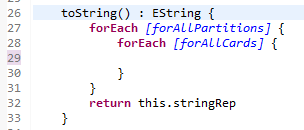
\includegraphics[width=0.5\textwidth]{eclipse_toStringNestedLoops}
  \caption{Control flow for \texttt{toString}}
  \label{fig:emptyLoops}
\end{center}
\end{figure}

\item[$\blacktriangleright$] In order to invoke \texttt{addToStringRep}, we need to make use of a new activity node type, a \emph{statement node}. These are
different from story patterns as they are able to invoke methods as part of the control flow. A statement node is declared by surrounding the invocation command
with  `\texttt{<>}.' Therefore, inside the second loop, write \texttt{<@this.addToStringRepCard(card)>}. The correct \texttt{card} parameter will be matched by
the \texttt{ForAllCards} pattern, which we'll establish next.

\vspace{0.5cm}

\item[$\blacktriangleright$] The \texttt{toString} activity should now resemble Fig.~\ref{fig:toStringFlow}.

\vspace{0.5cm}

\begin{figure}[htp]
\begin{center}
  \includegraphics[width=0.6\textwidth]{eclipse_boxtoStringFlow}
  \caption{Our first \emph{statement node}}
  \label{fig:toStringFlow}
\end{center}
\end{figure}

\item[$\blacktriangleright$] The aim of the activity to access every item in a \texttt{Box}. The control flow (which we've already established), invokes a
helper method to complete the action. This means both patterns need only match their object variables to ensure that all cards in all partitions are found.

\item[$\blacktriangleright$] Complete each pattern as depicted in Fig.~\ref{fig:toStringPatterns}. The \texttt{partition}in \texttt{forAllCards} is bound to
the current one matched in the first loop containing \texttt{forAllPartitions}, but \texttt{card} is \emph{not} bound as it must be matched with
\texttt{forAllCards.}

\vspace{0.5cm}

\begin{figure}[htp]
\begin{center}
  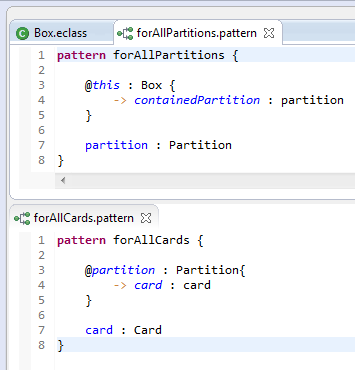
\includegraphics[width=0.6\textwidth]{eclipse_toStringPatterns}
  \caption{Box traversal patterns}
  \label{fig:toStringPatterns}
\end{center}
\end{figure}

\vspace{0.5cm}

\item[$\blacktriangleright$] As crazy at it may seem, that's it!  To see how this SDM is represented visually, check out Fig.~\ref{fig:sdm_tostring_5}.

\end{itemize}
